%%% LaTeX Template: Article/Thesis/etc. with colored headings and special fonts
%%%
%%% Source: http://www.howtotex.com/
%%% Feel free to distribute this template, but please keep to referral to http://www.howtotex.com/ here.
%%% February 2011
%%%
%%% Last updated September 2021 by CDM

%%%  Preamble
\documentclass[11pt,letterpaper]{article}
\usepackage[margin=1.0in]{geometry}
\usepackage[T1]{fontenc}
\usepackage[bitstream-charter]{mathdesign}
\usepackage[latin1]{inputenc}					
\usepackage{amsmath}						
\usepackage{xcolor}
\usepackage{cite}
\usepackage{hyphenat}
\usepackage{graphicx}
\usepackage{float}
\usepackage{subfigure}
\usepackage{sectsty}
\usepackage[compact]{titlesec} 
\usepackage[tablegrid]{vhistory}
\allsectionsfont{\color{accentcolor}\scshape\selectfont}

%%% Definitions
\definecolor{accentcolor}{rgb}{0.0,0.0,0.5} 
\newcommand{\teamname}{Team Name}
\newcommand{\productname}{Product Name}
\newcommand{\coursename}{CSE 4316: Senior Design I}
\newcommand{\semester}{Fall 2021}
\newcommand{\docname}{Project Charter}
\newcommand{\department}{Department of Computer Science \& Engineering}
\newcommand{\university}{The University of Texas at Arlington}
\newcommand{\authors}{Alan Turing \\ Grace Hopper \\ John Von Neumann \\ Ada Lovelace \\ Charles Babbage}

%%% Headers and footers
\usepackage{fancyhdr}
	\pagestyle{fancy}						% Enabling the custom headers/footers
\usepackage{lastpage}	
	% Header (empty)
	\lhead{}
	\chead{}
	\rhead{}
	% Footer
	\lfoot{\footnotesize \teamname \ - \semester}
	\cfoot{}
	\rfoot{\footnotesize page \thepage\ of \pageref{LastPage}}	% "Page 1 of 2"
	\renewcommand{\headrulewidth}{0.0pt}
	\renewcommand{\footrulewidth}{0.4pt}

%%% Change the abstract environment
\usepackage[runin]{abstract}			% runin option for a run-in title
%\setlength\absleftindent{30pt}			% left margin
%\setlength\absrightindent{30pt}		% right margin
\abslabeldelim{\quad}	
\setlength{\abstitleskip}{-10pt}
\renewcommand{\abstractname}{}
\renewcommand{\abstracttextfont}{\color{accentcolor} \small \slshape}	% slanted text

%%% Start of the document
\begin{document}

%%% Cover sheet
{\centering \huge \color{accentcolor} \sc \textbf{\department \\ \university} \par}
\vspace{1 in}
{\centering \huge \color{accentcolor} \sc \textbf{\docname \\ \coursename \\ \semester} \par}
\vspace{0.5 in}
\begin{figure}[h!]
	\centering
   	
\includegraphics[width=0.60\textwidth]{images/test_image}
\end{figure}
\vspace{0.5 in}
{\centering \huge \color{accentcolor} \sc \textbf{\teamname \\ \productname} \par}
\vspace{0.5 in}
{\centering \large \sc \textbf{\authors} \par}
\newpage


%\vspace{1 in}
%\centerline{January 13th, 2012}
%\newpage

%%% Revision History
\begin{versionhistory}
  	\vhEntry{0.1}{10.01.2021}{GH}{document creation}
  	\vhEntry{0.2}{10.05.2021}{AT|GH}{complete draft}
  	\vhEntry{0.3}{10.12.2021}{AT|GH}{release candidate 1}
  	\vhEntry{1.0}{10.20.2021}{AT|GH|CB}{official release}
  	\vhEntry{1.1}{10.31.2021}{AL}{added customer change requests}
\end{versionhistory}
\newpage

%%% Table of contents
\tableofcontents
\newpage

%%% List of figures and tables (optional)
\listoffigures
%\listoftables
\newpage
\setcounter{table}{0}

%%% Executive summary sections
\section{Problem Statement}

There are many reasons why we want to create the ThereMelo, and one of them is to exercise our musical interests. This project is also a great gateway to show the younger generation about STEM-related projects in a fun way. We want to show there is much more than just standard projects. 

Computer vision is integrating itself into our society every passing day. We aim to integrate the use of computer vision into the field of music which also has a great impact on our daily lives. ThereMelo is a way to create music that will make it more accessible to those who may not have the ability as a result of the current state of music creation. All someone needs to have access to is a camera in order to realize their creative musical ideas.

Our aim is also to inspire the younger generation to take up an interest in STEM. We believe it is the job of the older generation to show the capabilities and to inspire others that STEM should be something that is fun and educational. That it can be more than just it seems.
\section{Methodology}
We are going to be creating software which will use the users camera and convert their hand movement into sound. Our software would simulate how a real theremin would work, where the users' dominant hand would be calculated in relative to their non-dominant hand to produce sound. The application would allow the user to enter a sandbox environment, where they are able to use the theremin however they want, or follow along in a few interactive tutorials to learn how to play the instrument with some selected songs.
\section{Value Proposition}
Our work should be funded because we want to introduce our application to younger generations to inspire them into STEM, mainly Computer Science. Our current sponsor, Shawn N. Gieser, also suggested that as well. This is beneficial, as the project may jump-start a new generation of STEM students. Music is highly influential, so lending the application to the audience may pique their interest in how the application manages to translate their hand movements into sound, which can produce music. 
\section{Development Milestones}
This list of core project milestones should include all major documents, demonstration of major project features, and associated deadlines. Any date that has not yet been officially scheduled at the time of preparing this document may be listed by month.
\\
\\
Provide a list of milestones and completion dates in the following format:
\begin{itemize}
  \item Project Charter first draft - September 2023
  \item System Requirements Specification - October 2023
  \item Architectural Design Specification - November 2023
  \item Demonstration of sound produced from user - February 2024
  \item Detailed Design Specification - Month Year
  \item CoE Innovation Day poster presentation - April 2024
  \item Final Project Demonstration - May 2024
\end{itemize}

%%%\item Demonstration of <feature or implementation milestone> - Month Year
\newpage

%%% Remaining project charter sections
\section{Background}
\quad We are given an opportunity from our sponsor, Shawn N. Gieser to create a virtual theremin so we jumped onto this chance. This project was brought up from him during a meeting and we wanted this project. With this project is allows us to use our love for music to create a unique instrument that is not reliably available to most people. 

\quad A theremin, for those who do not know, is an instrument that does not require any touch, but it uses the players hand to change a magnetic field to create sound. When it comes to playing the user's non-dominant  hand is used to control the volume of the instrument while the dominant  is used to control the pitch. It both the sound and the act of playing the instrument is unique. Most people do not know what this instrument is and we would like to show a broader spectrum of people to it. 

\quad Since we want more people to be able to try out the theremin we want to allow for our software to be open to anyone. This will allow for anyone online to be able to grab our software and run it on there machine as long as they have a Leap Motion Controller 2. Our project exist to allow for any individual to be able to learn a theremin without the need to purchase one. We believe that the instrument should receive a lot more attention, but we understand that the issue with a real theremin is the cost of one it quite expensive. We can stop cost of entry this with our product making it cheaper than a real theremin.

\quad Along with making it cheaper we can use our project as a point of inspiration for the younger generation. Our sponsor has had the idea that we should make this project with the thought of kids involved so that this project is capable to show what people can do with computer science. This would an amazing example of what the world of computer science is capable and allow for a new generation of computer scientist. We feel as inspiring the next generation is more than enough of a reason for a project to exist cause it is like an art. We would like for our project to be show around the state of Texas. Our sponsor feels the same way as we do to our knowledge.

\quad Our sponsor is our teacher and we are their students. We have talked a little bit about the expectation from our project and has even recommend us our current hand tracker. We will be going to them for guidance when we need a guiding hand to help us along when we will needed. This is sorta of a dream project were we can work on something that allows for creative freedom and can inspire others into the same field that we fell in love with. 

\section{Related Work}

In the realm of hand-tracking technology, the "state-of-the-art" has seen significant advancements in recent years, offering various solutions across different domains. These solutions vary from academic research prototypes to commercially available products. In the context of your project, which aims to create a hand-tracking program for music generation similar to playing the theremin using the Leap Motion camera and advanced software, it's essential to survey the existing landscape and understand why these solutions may not fully meet your customer's needs.

The landscape of hand-tracking technology has undergone rapid and extensive transformations in recent times. Notably, there are innovative devices that employ "free-space, unencumbered hand-tracking using an array of distance sensors" \cite{Chronopoulos2021}, alongside various other cutting-edge techniques. In our pursuit of advancing ThereMelo, we aim to seamlessly integrate these evolving techniques, unlocking new possibilities and applications to take the hand-tracking experience to the next level.

Hand-tracking technology has found diverse applications in today's world, with one prominent domain being the medical industry. An illustrative case in point is its application in "surgical telestration" \cite{Muller2022}, where surgeons can benefit from precise hand-tracking for enhanced surgical procedures. However, despite its widespread utility, hand-tracking hasn't seen as much adoption in the realm of music and entertainment. This is where ThereMelo comes into play. Our mission is to harness the power of ThereMelo to bridge this gap and bring the captivating world of music interaction to the general public, making it more accessible and engaging.

Devices such as the Leap Motion camera \cite{Vysocky2020} are pioneers in hand-tracking technology. Their device, the Leap Motion Controller, offers precise hand and finger tracking. However, while it provides high-quality data, it might not be optimized for the specific musical interaction you're envisioning. It primarily focuses on gesture recognition rather than music generation. This is precisely why we aim to use their newest technology, Leap Motion 2, and ThereMelo in collaboration to help bridge this gap.

There are current devices that, similar to ThereMelo, will take in motion-tracking data and process it in order to manipulate music. "Users can easily
control music equipment and achieve high accuracy of music control information." \cite{Pan2021} But the use cases for these current systems are used for things like pause/play functions. The ThereMelo will take these functions and expand on their usefulness to include things like changing pitch, volume, and notes.

Included in this application of hand-tracking to music is the "use of a gesture-based inter-action game as an entertainment system but, also as a hand-tracking evaluation tool." \cite{Figueiredo2012}. These systems are not currently tailored to the creation and expressive freedoms that are allowed by the use of physical instruments. This is the main purpose for our advancement of ThereMelo. We expect this new technology to not only make the music and entertainment industry more accessible to those who seek it but also to make the interaction between humans and music more engaging.

Limitations that might exist for the existing solutions can include:

1.) Costs- The actual commercial theremins that exist in the market can be very expensive for many users. Music and theremin enthusiasts might be looking out for an alternate affordable option.



\section{System Overview}

We will be implementing software that will utilize a hand tracker and your laptop/desktop. What is expected of the user is to have the hand tracker, which will send information about the user's hands to their device. After the information is sent to the device, our software will read that information and react accordingly to their gestures, height, and distance.

Our program will be able to take data from the provided hand tracking software and manage the hands' positions. We will then ask the user to show their dominant hand, in order for the software to figure out their hand space. With the calibration completed, we can convert their motions into sound, which will play on their device's speakers.

The program will also ask the user if they want to in a sandbox environment or a learning environment. The sandbox environment will allow the user to play the ThereMelo without many restrictions, just like a regular instrument. The learning environment will allow the user to learn how to play the instrument, and learn a couple of songs along the way.

Our main controls is the user's non-dominant hand will control the instrument's volumes and their dominant hand will determine the pitch. With this we can convert the input from the user and turn it into sound which will mimic the theremin. 

\begin{figure}[h!]
	\centering
   	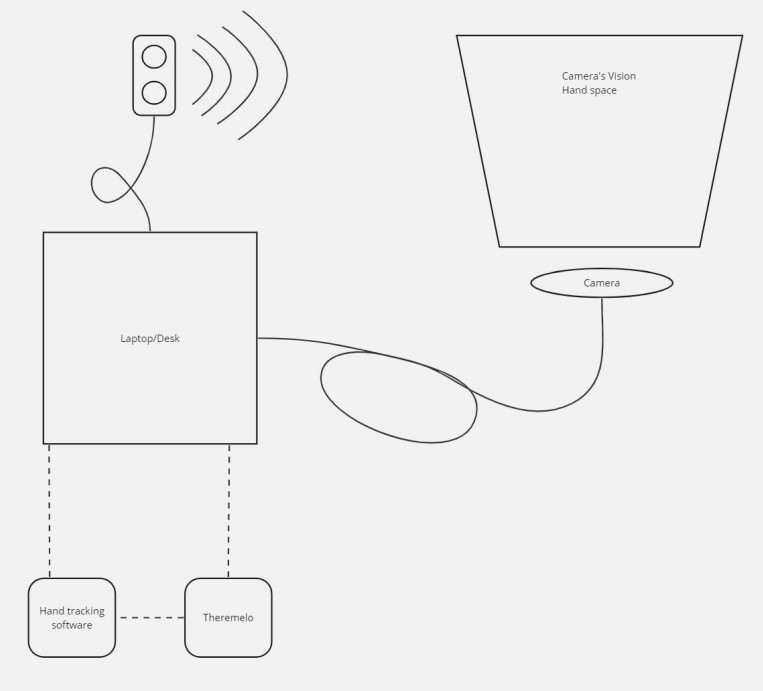
\includegraphics[width=0.8\textwidth]{images/systemOverview.jpg}
    \caption{System Overview}
\end{figure}

\section{Roles \& Responsibilities}
Currently, we have no sponsors for our project other than our professor. Our team member consists of Scott Frazier, Ron Nguyen, Farhan Sadiq, Sazzadul Islam, and Caleb Myatt.

The stake holders in our project is our sponsor and teacher Shawn N. Gieser and the team including Scott Frazier, Ron Nguyen, Farhan Sadiq, Sazzadul Islam, and Caleb Myatt. Caleb is the point of contact to our sponsor. We will go about each individual what they want to do and take on that areas responsibility. 

Caleb will take on the role as the point of contact, and work on the coding side of the hands. What this will include with responsibilities is being able to contact with sponsor and telling our needs to him. Other responsibilities would also include getting the hand input from the user and converting that into our desired sounds. 

Ron will focus on working with the hand and the User Interface. This will include the responsibilities of converting the hand input from the user and converting  that into our desired sounds. Also they will be creating an interface for the end user to be able to interact with our software. 

Farhan will also focus on the coding aspects of the hands. This will include mostly backend work. He will also be assisting in any documentation work required for the project.

Sazzadul will also be focusing on coding and testing aspects of the project. This will include collaborating with the team on the coding aspects, particularly focusing on specific features or functionalities that require development and testing. Also, contribute with the team members for any documentation needed for the project.    

Scott will be focusing on documentation and testing of the hands. This will include talking to the team and understanding the project as a whole. The testing of the hands will be manually to ensure a good end user experiance. 

Our scrum master will change periodically when we feel like there is a need of change so that we can take a different approach. 

\section{Cost Proposal}
This section contains the approximate budget for the project, where that money will come from, and any other support. This text should be replaced with a discussion and justification of major expenses, but not the actual monetary amounts (that will go in the preliminary budget section below). 

Our budget is fairly cheap. Our main purchase will be the Leap Motion Controller 2 by Ultraleap. Since our project will require hand tracking to simulate a theremin, it will be easier to an existing hardware to keep track of the hand positions with IR. We are currently looking at Plastic SCM as an alternative to GitHub, as they have a limit of 2 GB for our plan. Only issue we can see is that Plastic SCM is a paid service for teams of 5, so we may need to discuss more if we were to migrate.

\subsection{Preliminary Budget}
Include a high level budget table for components, fabrication, software licensees, development hardware, etc. This should be in a tabular format broken up into appropriate line items. 
\begin{center}
\begin{tabular}{|l|l|l|}
\hline
\textbf{Item} & \textbf{Description} & \textbf{Price}  \\ \hline
Leap Motion Controller 2 & IR Camera, tracks user hands. Made by Ultraleap & \$139  \\ \hline
Plastic SCM & Unity's Version Control. Paid monthly if ever used. & \$14  \\ \hline
\end{tabular}
\end{center}


\subsection{Current \& Pending Support}

\begin{center}
\begin{tabular}{|l|l|}
\hline
\textbf{Provider} & \textbf{Price}  \\ \hline
CSE department &  \$550  \\ \hline
Scott Frazier &  \$50  \\ \hline
Ron Nguyen &  \$50  \\ \hline
Farhan Sadiq &  \$50  \\ \hline
Sazzadul Islam &  \$50  \\ \hline
Caleb Myatt &  \$50  \\ \hline

\end{tabular}  
\end{center}

\section{Facilities \& Equipment}
We would need a dedicated lab space that has enough room for us to setup the camera to work on our project. We need the lab/testing space to have sufficient lighting conditions and an open area where we could carry out our tests for the project. The lab space should be free from any sort of interference that might the disrupt the performance of the UltraLeap. 

Our project requires hand tracking to simulate a theremin, so our main purchase would be the Leap Motion Controller 2 by UltraLeap. We plan to use Unity development software and licenses, to create the theremin's virtual interface. We will use GitHub, to collaborate and work on the program together as a team. We might migrate over the Plastic SCM if the repository fills up. That would require a payment service. We have a group on Discord, which is our main platform to communicate and discuss about the projects.


\section{Assumptions}
The following list contains 5 critical assumptions related to the implementation and testing of the project.

\begin{itemize}
  \item Our hand tracker will be delivered somewhere between the 1st sprint cycle.
  \item Our Unity environment will be stable for both Windows and Mac around the beginning of the 2nd sprint cycle.
  \item Basic user interface will be completed by the 3rd sprint cycle.
  \item Application's sound engine should be functional near the end of 3rd sprint cycle.
  \item Unity's Terms of Service won't update to hinder our project in the near future.
\end{itemize}
\section{Constraints}
The following list contains 5 key constraints related to the implementation and testing of the project.

\begin{itemize}
  \item Final prototype demonstration must be completed by May 1st, 20XX
  \item Total development costs must not exceed \$800.
  \item Limit gestures and motions for simplicity.
  \item Additional time must be spent on learning and skill development.
  \item Regression testing must be ensured after any updates or changes, to test the correct working of existing functionalities.
\end{itemize}

\section{Risks}
The following high-level risk census contains identified project risks with the highest exposure. Mitigation strategies will be discussed in future planning sessions.

\begin{table}[h]
\resizebox{\textwidth}{!}{
\begin{tabular}{|l|l|l|l|}
\hline
 \textbf{Risk description} & \textbf{Probability} & \textbf{Loss (days)} & \textbf{Exposure (days)} \\ \hline
 GitHub Repository hits max capacity & 0.45 & 14 & 6.3 \\ \hline
 Unity Environment malfunctioning & 0.25 & 20 & 5.0 \\ \hline
 Compatibility Issues & 0.25 & 10 & 2.5 \\ \hline
 Failure to tune in desired musical tones & 0.15 & 10 & 1.5 \\ \hline
 Leap Motion Controller 2 non functional  & 0.10 & 10 & 1.0 \\ \hline
 
\end{tabular}}
\caption{Overview of highest exposure project risks} 
\end{table}
\section{Documentation \& Reporting}
%%% In this section, you will describe all of the various artifacts that you will generate and maintain during the project life cycle. Describe the purpose of each item below, how the content will be generated, where it will be stored, how often it will be updated, etc. Replace the default text for each section with your own description. Reword this paragraph as appropriate.

\subsection{Major Documentation Deliverables}

\subsubsection{Project Charter}

We will be maintaining this project charter during all sprints. Usually near the end once we get a better understanding of what we have accomplished then update it. The initial version of our project charter will come out once our product has reached testing phase, and the final version will be once we have everything working. 

\subsubsection{System Requirements Specification}

We will be updating System Requirements specifications anytime we have a major change in our project like a shift in languages or hardware. The initial version should come out once we have our finished product and working on distribution. 

\subsubsection{Architectural Design Specification}

This document will be maintained near the end of sprints so we can take a look back and be able to properly explain how we built it. We will have a meeting talking about how we will got about the architectural and compare it to the finally result and check they are the same. This will be delivered along side of the Project Charter so that anyone can see our Design process in understanding what we did.


\subsubsection{Detailed Design Specification}

This document will be maintained alongside the Architectural due to the similarities between the documents. We will be following the same process when we update this document and Architectural Design. 

\subsection{Recurring Sprint Items}



\subsubsection{Product Backlog}

The items will be add to the SRS by when we need to add. The items will be prioritized based on due dates from sponsor and then what can be done within the sprint. Decision are left to a vote when capable. We will be using excel for our product back log. 


\subsubsection{Sprint Planning}

Each sprint, we'll plan on Monday that starts our sprint, then every Friday, we meet together to collaborate. We will also tend to meet on weekends virtually as well for collaboration. We will be having four sprints this semester, and possibly another 4 more sprints for the next semester.

\subsubsection{Sprint Goal}

Our sprint goal is decided by our sponsor currently, and as a group. We will ask friends what they would want from this software for ideas but in the end it is up the group.

\subsubsection{Sprint Backlog}

With the meeting on Friday we will decide what goes onto the sprint back log, and the backlog will be maintained by everyone on excel.

\subsubsection{Task Breakdown}

Everyone will voluntarily claim task and we will document our time on our backlog.

\subsubsection{Sprint Burn Down Charts}

Caleb will be responsible for generating the burn down chart for each sprint. They will take from the backlog and take the time expected to finish all of the work and document each day about how much was done. The format is just a simple line (Red line) from expected effort to 0, and then our document line (blue line) showing what we have done.

\begin{figure}[h!]
    \centering
    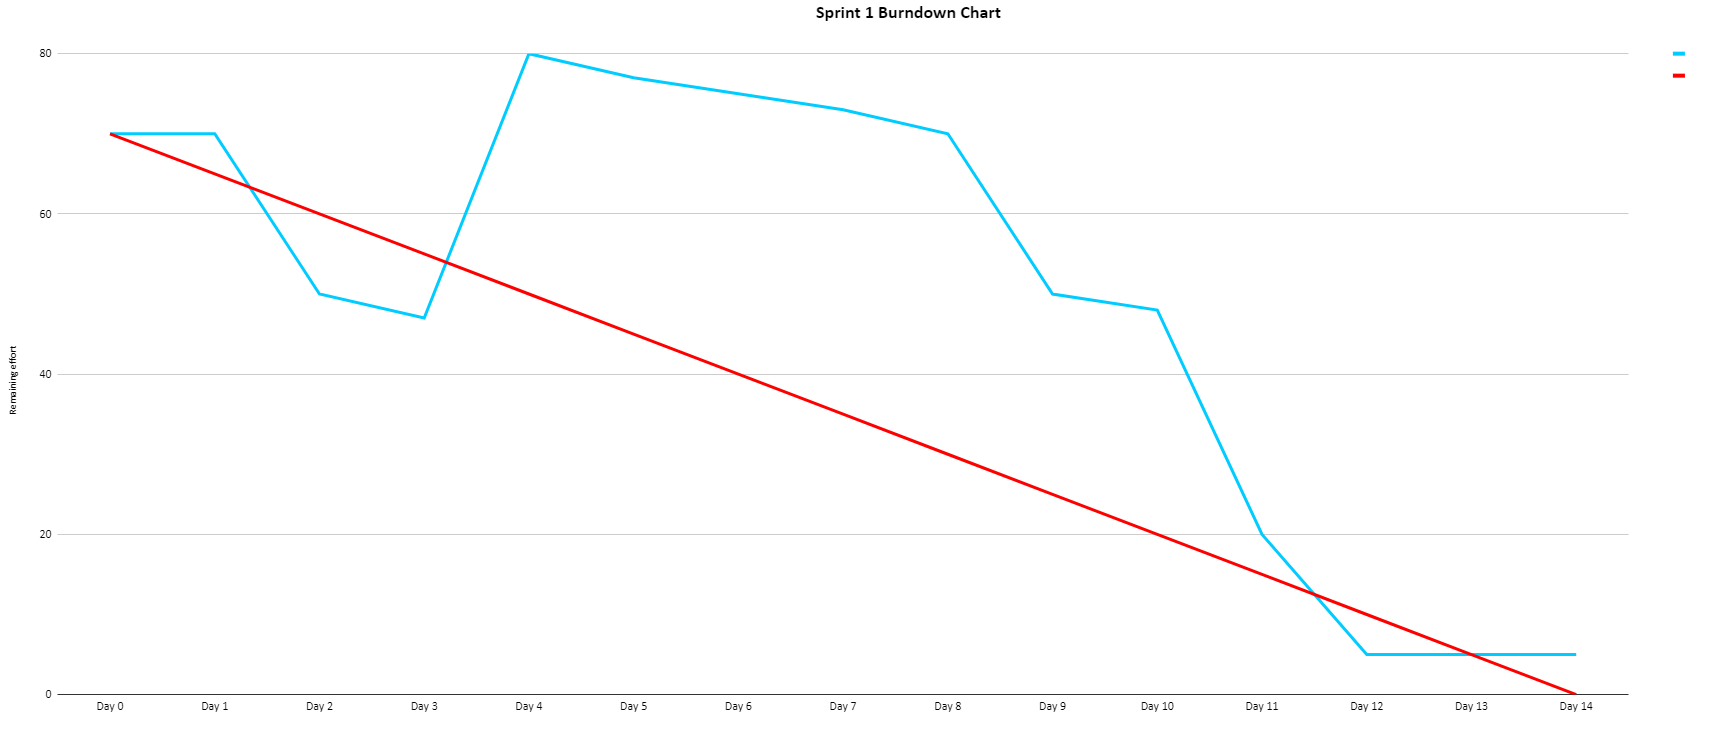
\includegraphics[width=0.8\textwidth]{images/ExampleSprint}
    \caption{Example sprint burn down chart}
\end{figure}

\subsubsection{Sprint Retrospective}

On the Friday, after the sprint is done, we will talk about what has happen. The individual will document what they have done for each task where the group is documented based on the deliverables and documentation. 

\subsubsection{Individual Status Reports}

Everyone will been given the same status up, and it will be reported on after the sprint. The key items is our sprint goals, backlog, Individual time expenditures, team burn down chart, individual retrospectives, and a peer review. 

\subsubsection{Engineering Notebooks}

We do not plan to use an Engineering note book. That is up the the individual if they wish to do that.

\subsection{Closeout Materials}

\subsubsection{System Prototype}

In our final system prototype we expect the have the software being able to have a lesson plan, and sandbox mode. We want the user to be able to learn how to use the ThereMelo within and have fun with it. 


\subsubsection{Project Poster}

The Poster will just be a tri-fold presentation board and it will just have who we are and what are product is. 

\subsubsection{Web Page}

For our web page we would want to post everything and we want it to be accessible to the public. This will be provided at the end once our product is completed. 

\subsubsection{Demo Video}

We will show the process/ behind the scene of the game as B-reel footage while we explain how our software works. The video should only be around 3 minutes and it will just cover how our product works and run a simple lesson. 

\subsubsection{Source Code}

We will be using GitHub as our version control system. We plan to have our software to just be binaries but we would like to also include the source code. The product will be open sourced for the general public at the end and we will be using GNU GPL for our license. It will be all in the LICENSE in main. 

\subsubsection{Source Code Documentation}

We will be using Doxygen and we will have it as a pdf.

\subsubsection{Hardware Schematics}

We do not have any hardware so this is not applicable to us

\subsubsection{CAD files}

We do not have any CAD files so this is not applicable to us

\subsubsection{Installation Scripts}

We will try to use Unity as a way to allow for user to download it. 

\subsubsection{User Manual}

We will create a digital user manual, but it is not likely needed to the program should be able to run as long as the camera and any other software is already downloaded. 
\newpage

%%% References
\bibliographystyle{plain}
\bibliographystyle{reference/IEEEtran_custom}
\bibliography{reference/refs}{}

\end{document}